\documentclass[a4paper,11pt]{article}
\usepackage{amsmath, amssymb, amsfonts, graphicx, hyperref, cite, array}
\usepackage{geometry}
\usepackage[T2A]{fontenc} % Font encoding
\usepackage[russian]{babel} % Russian language support
\usepackage{fontspec}
\usepackage{listings}
\usepackage{hyperref}
\usepackage{lmodern}
\usepackage{xcolor}
\usepackage{caption}
\usepackage{import}
\usepackage{array} % Для выравнивания по правому краю

% Import images from images/
\graphicspath{{images/}}

% Custom color definitions
\definecolor{lightestgray}{rgb}{0.95,0.95,0.95} % Lighter background color
\definecolor{darkblue}{rgb}{0.0,0.0,0.5} % Darker blue for keywords
\definecolor{darkgreen}{rgb}{0.0,0.5,0.0} % Darker green for comments
\definecolor{darkred}{rgb}{0.5,0.0,0.0} % Darker red for strings

\setmainfont{Times New Roman}

\hypersetup{
    hidelinks % Полностью убирает рамки и цвет ссылок
}


% Custom label for listings
% \renewcommand{\lstlistingname}{Листинг кода}
% \renewcommand{\lstlistlistingname}{Список листингов}

% Define Julia language settings
\lstdefinelanguage{Julia}%
  {
	morekeywords={abstract,break,case,catch,const,continue,do,else,elseif,%
		end,export,false,for,function,immutable,import,importall,if,in
		macro,module,otherwise,quote,return,switch,true,try,type,typealias,%
	using,while},%
	basicstyle=\ttfamily, % Basic style is monospace
	showstringspaces=false, % Do not show spaces in strings
	breaklines=true, % Automatically break long lines
	% extendedchars=true % Enable extended characters 
	frame=single, % Add a frame around the code
  	sensitive=true,%
   	alsoother={$},%
   	morecomment=[l]\#,%
   	morecomment=[n]{\#=}{=\#},%
   	morestring=[s]{"}{"},%
   	morestring=[m]{'}{'},%
}[keywords,comments,strings]%

\lstset{%
    language         = Julia,
    basicstyle       = \ttfamily,
    keywordstyle     = \bfseries\color{blue},
    stringstyle      = \color{magenta},
    commentstyle     = \color{darkgreen},
    backgroundcolor  = \color{lightestgray},
    showstringspaces = false,
}

\geometry{a4paper, margin=1in}
\title{Multiscale modeling 2}
\author{Panov Mikhail}
\date{\today}

\begin{document}

\maketitle
\tableofcontents
\newpage


\section{Part 1}
I ran scripts from [this link](https://group.miletic.net/en/tutorials/gromacs/1-tip4pew-water/) and processed the output to get images of potential energy, temperature, pressure, and diffusion coefficient.

\subsection{Graphs}
Scales are not the same as in examples but shapes of the graphs look correct.
\begin{figure}[htbp]
    \centering
    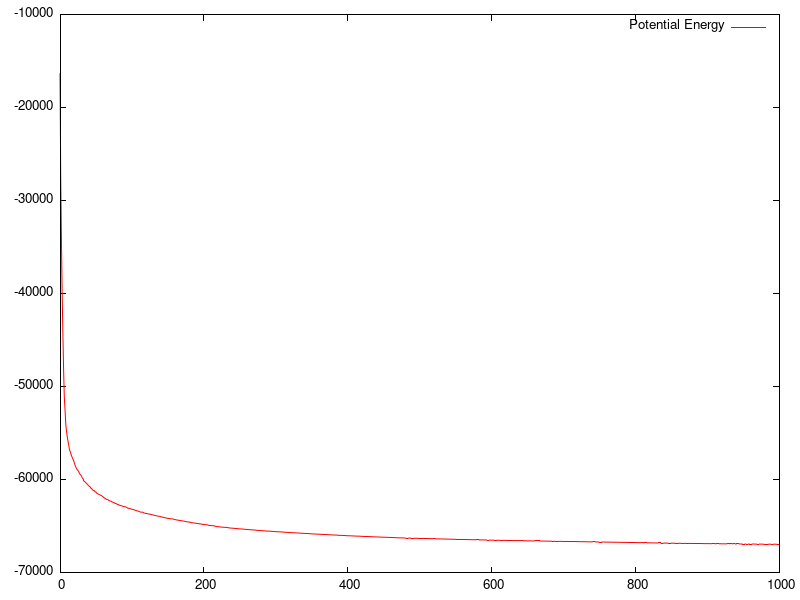
\includegraphics[width=0.45\textwidth]{min-energy.png}
    \caption{Potential Energy 1}
    \label{fig:pot_energy1}
\end{figure}

\begin{figure}[htbp]
    \centering
    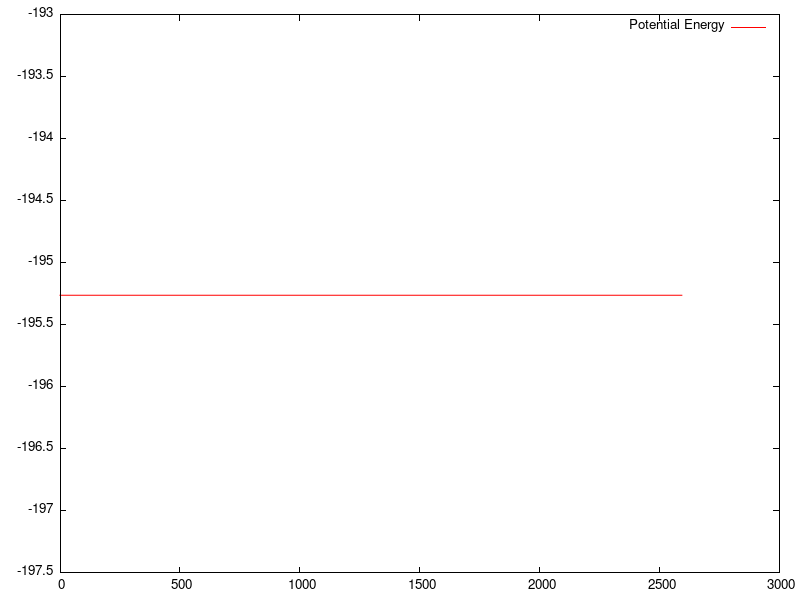
\includegraphics[width=0.45\textwidth]{min2-energy.png}
    \caption{Potential Energy 2}
    \label{fig:pot_energy2}
\end{figure}

\begin{figure}[htbp]
    \centering
    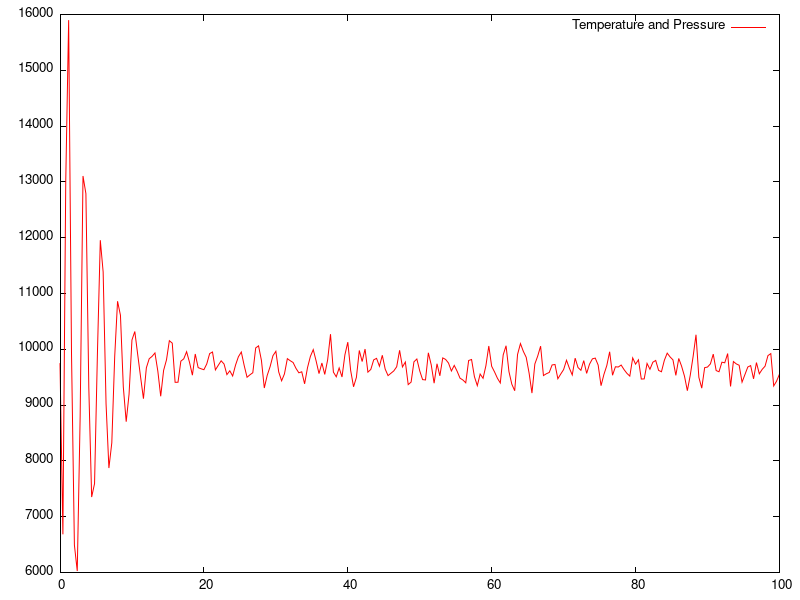
\includegraphics[width=0.45\textwidth]{eql-temp.png}
    \caption{Temperature}
    \label{fig:temperature}
\end{figure}

\begin{figure}[htbp]
    \centering
    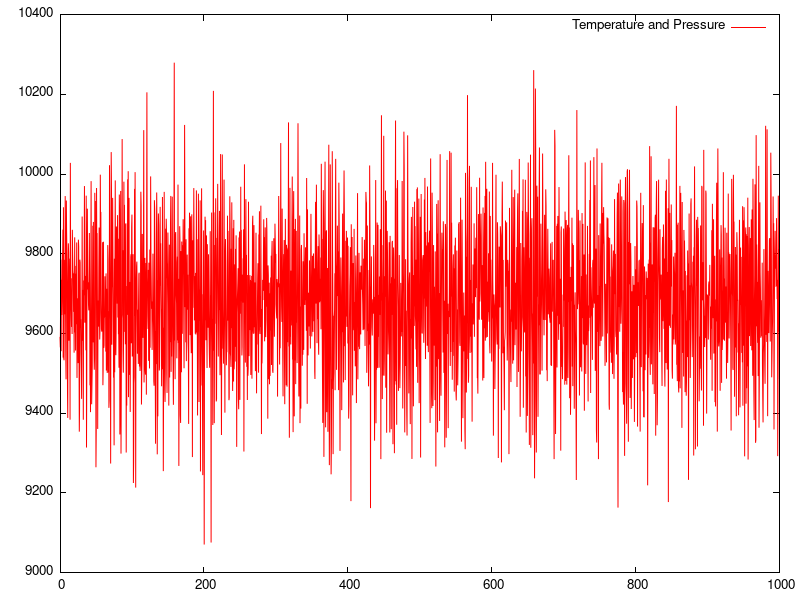
\includegraphics[width=0.45\textwidth]{eql2-temp.png}
    \caption{Pressure}
    \label{fig:pressure}
\end{figure}

\begin{figure}[htbp]
    \centering
    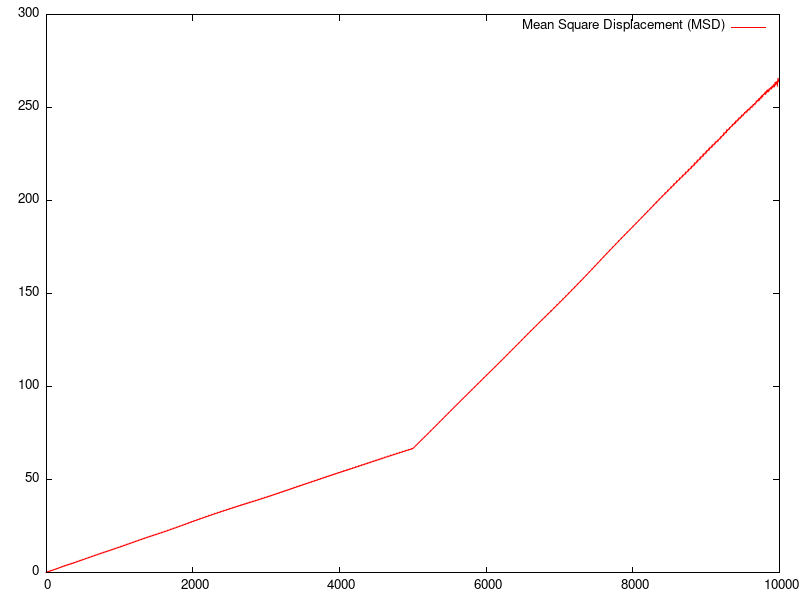
\includegraphics[width=0.45\textwidth]{prd-msd.png}
    \caption{Diffusion Coefficient}
    \label{fig:diff_coeff}
\end{figure}
\newpage

\subsection{Output Files}
Output SLURM files should be attached to the PDF. If any additional files, such as SBATCH, bash, or configuration files, are needed, they are available on the supercomputer and can be provided upon request.

\section{Part 2}
Results are mostly strange. One core performances are better than any multicore probes by far. All jobs showed very bad scale with number of cores. Single core results are not showed on the graphs below because they would be so high that all other scores would be indistinguishable.

\begin{figure}[htbp]
    \centering
    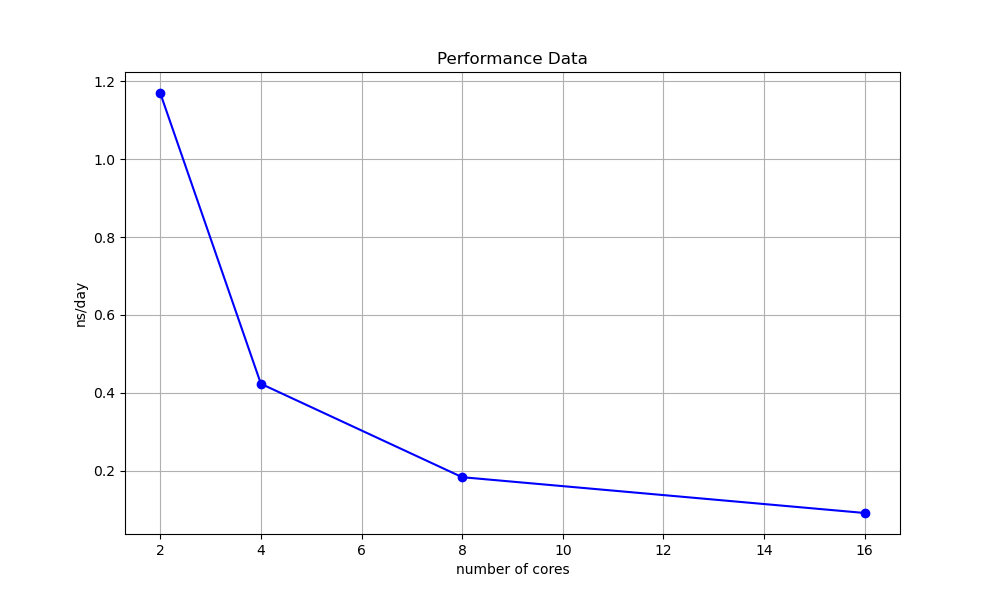
\includegraphics[width=0.45\textwidth]{job_error_strong.png}
    \caption{Strong scaling}
    \label{fig:strong}
\end{figure}

\begin{figure}[htbp]
    \centering
    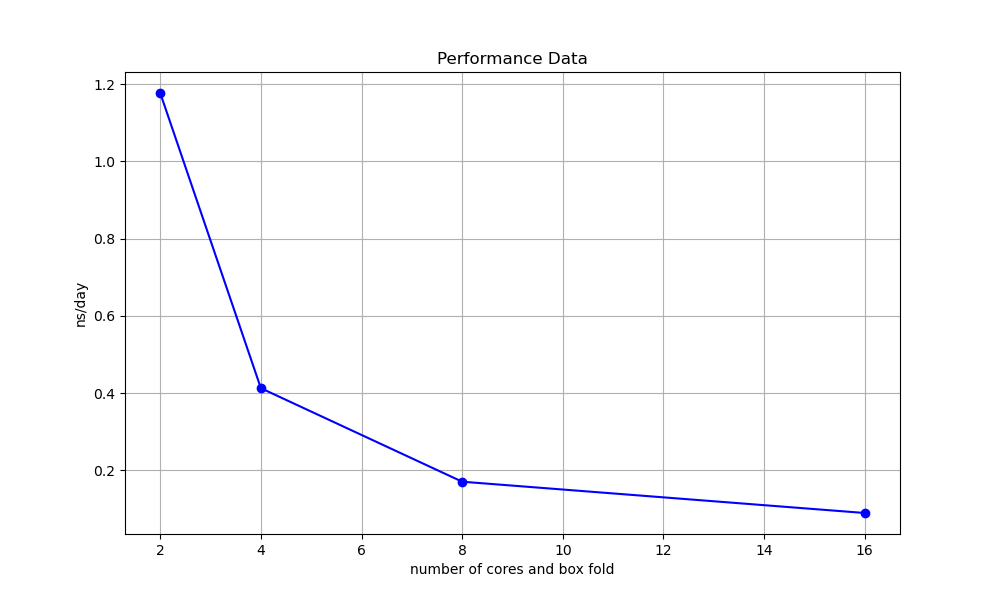
\includegraphics[width=0.45\textwidth]{job_error_weak.png}
    \caption{Weak scaling}
    \label{fig:weak}
\end{figure}

\begin{figure}[htbp]
    \centering
    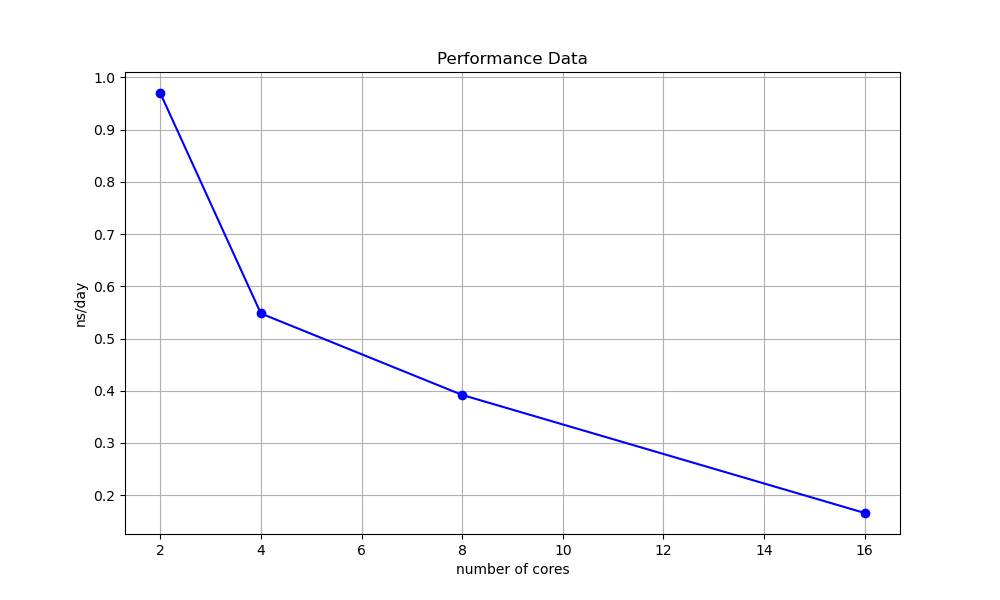
\includegraphics[width=0.45\textwidth]{job_error_fixed_gpu.png}
    \caption{Fixed 18832 particles GPU}
    \label{fig:fixed_gpu}
\end{figure}

\end{document}
